\section{Other Insights}

\subsection{Predict the medal of the 2032 Olympics}

\begin{figure}[h]
\centering
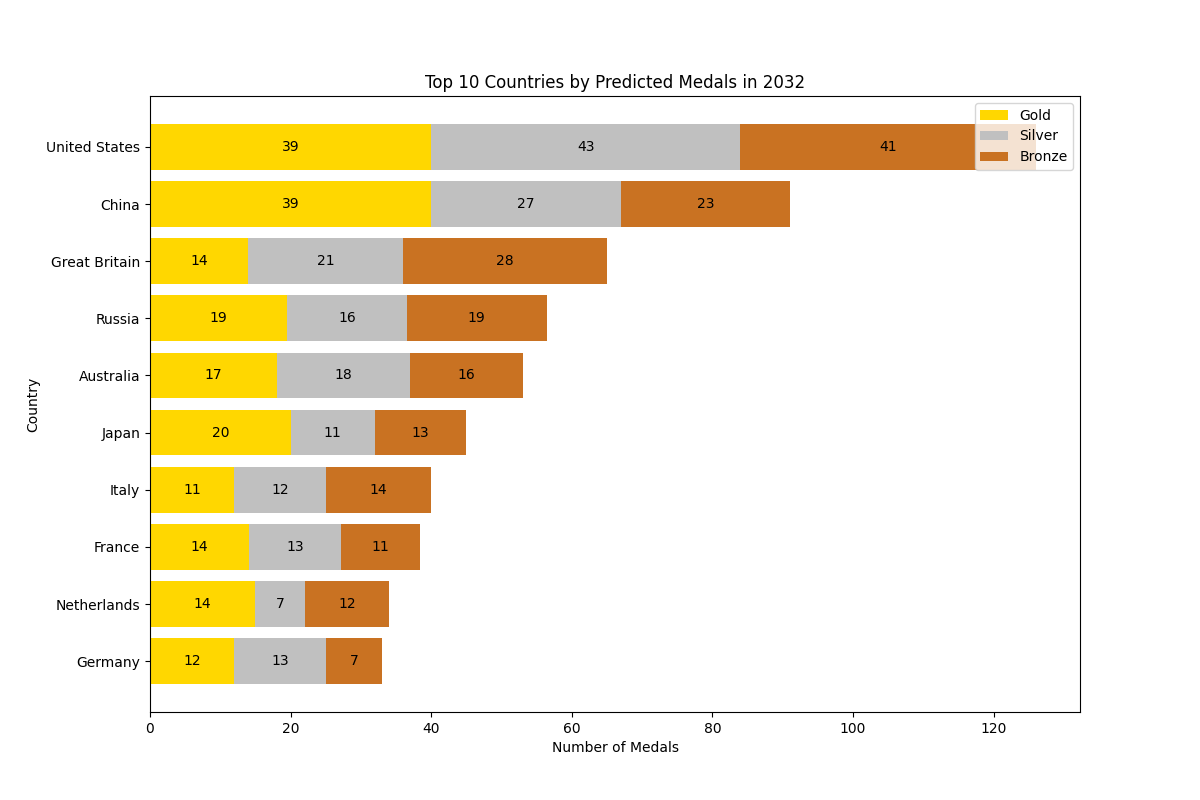
\includegraphics[width=1\textwidth]{../figures/2032.png}
\caption{Predicted Medal Counts for the 2032 Olympics}
\label{fig:medal_prediction}
\end{figure}

The prediction of 2032 Olympics is rather difficult because of the uncertainty of the future and almost no information of the 2032 Olympics. In \textbf{Figure \ref{fig:medal_prediction}}, we've tried to make some prediction with our comprehensive PRE model, taking all effects into account.Although the prediction may not be accurate enough, it can still serve as a reference.

\subsection{Greatness and the strategy of the country Olympic committees}
During the estimation of whether a country's achievement can be due to \textbf{Great Coaches}, we set a a parameter of \textbf{legendary} to evaluate the successness of a team on a certain event.
Combined with the \textbf{Great Athletes} mentioned before, we can now tell apart whether it's the great athlete(s) or the great coach that mainly contribute to great achievements.
Also, we can exclude these factors to more explicitly discuss other elements which influence various countries' performance.
\begin{figure}[h]
    \centering
    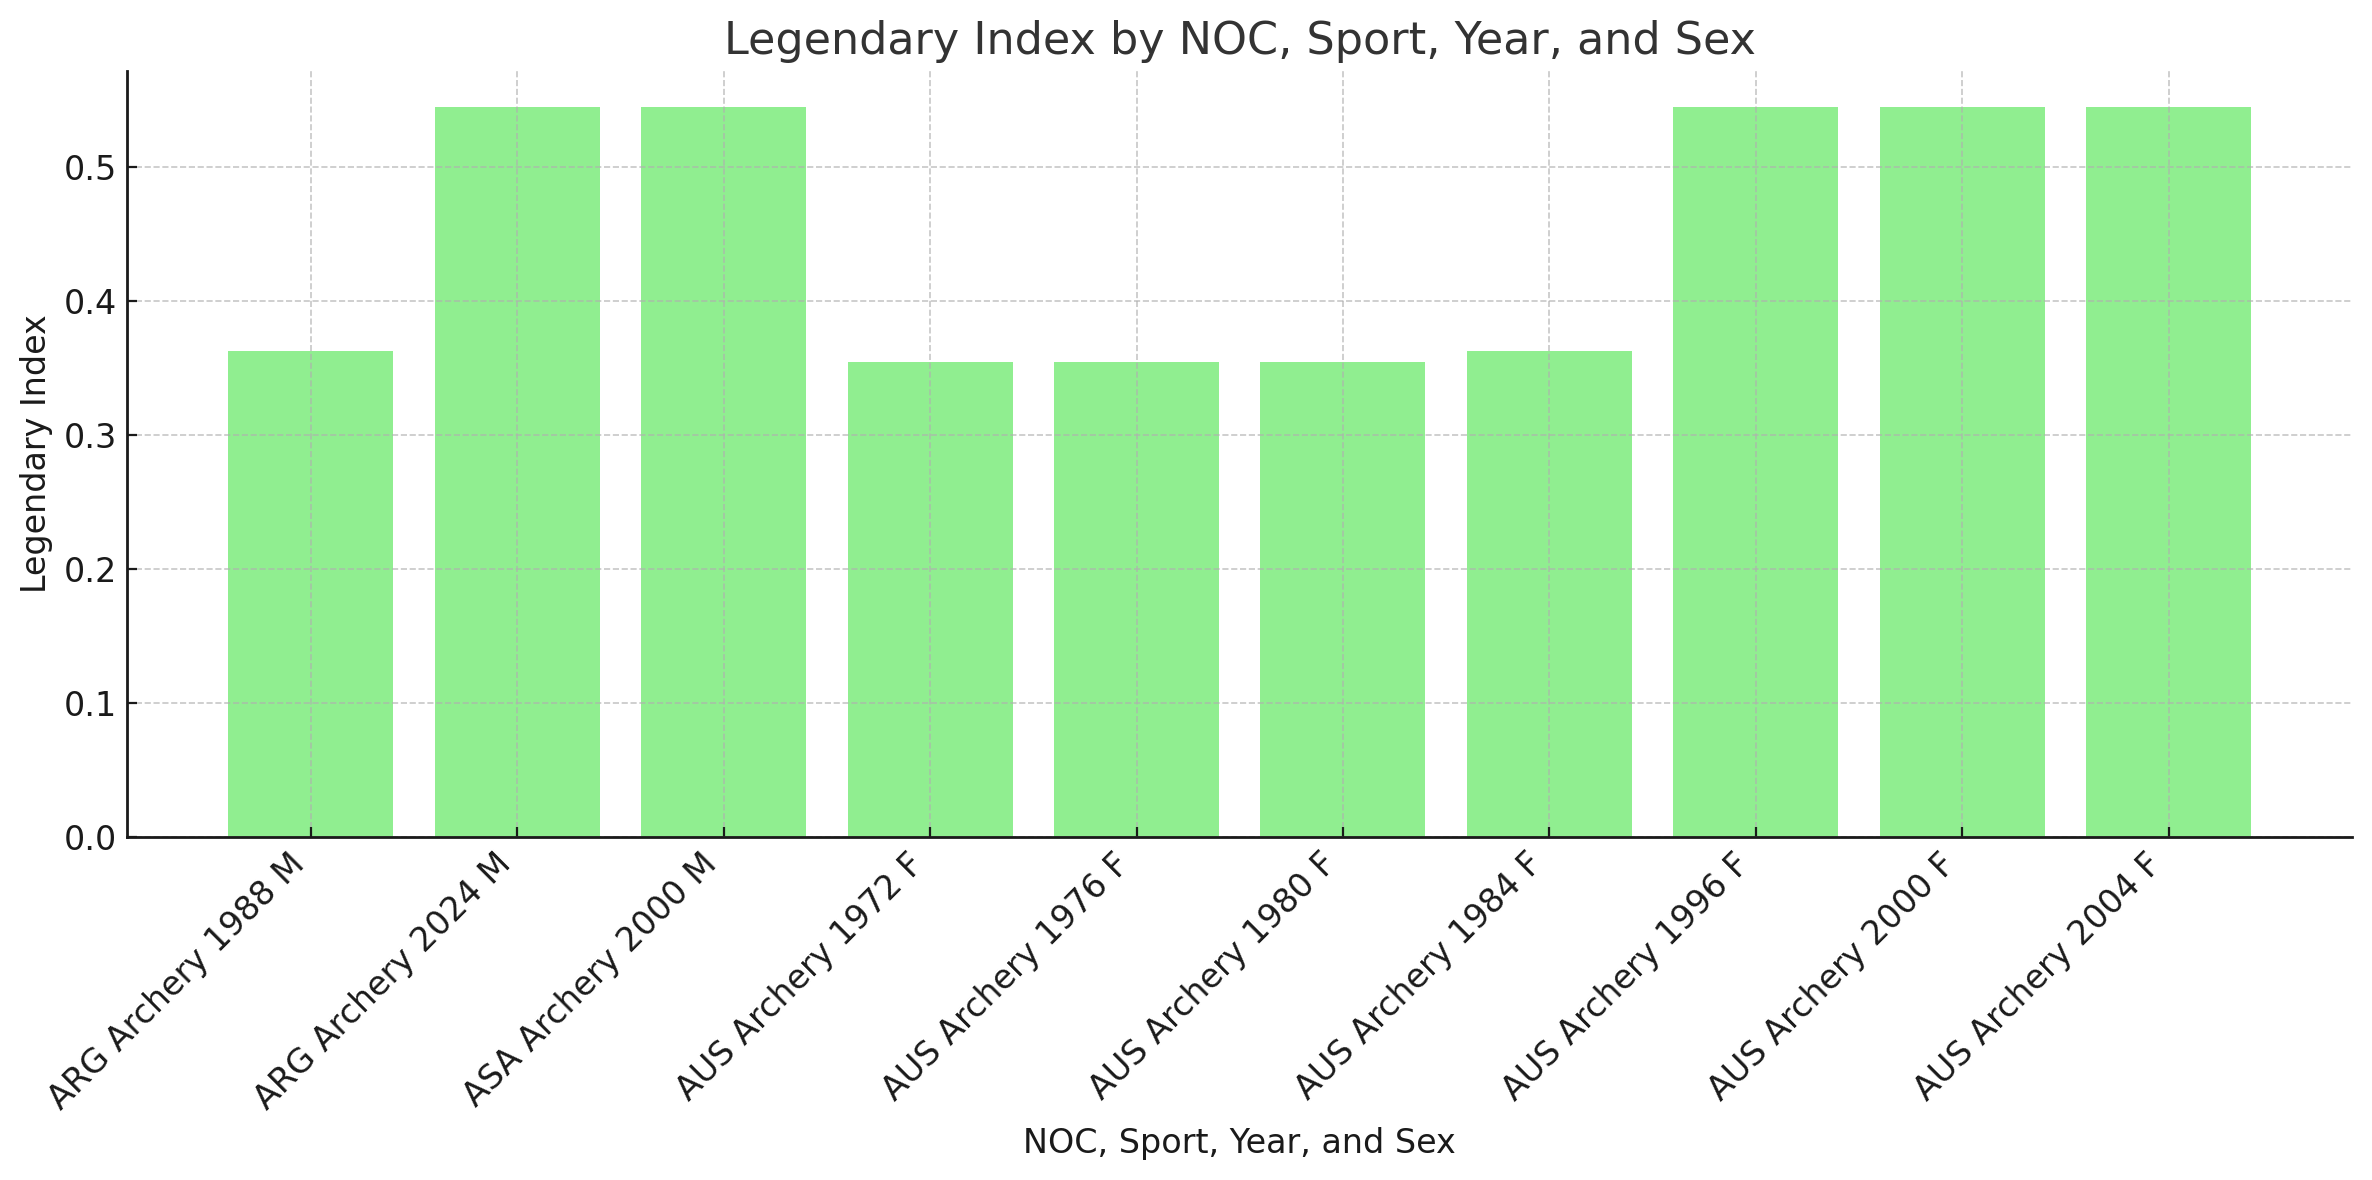
\includegraphics[width=1\textwidth]{./figures/Legendary_index.png}
    \caption{Legendary index of certain events}
    \label{fig:legendary_index}
    \end{figure}
The graph above shows a part of the calculation result. We find out that a high \textbf{legendary index} is of higher probability be due to \textbf{Great Coach} when a \textbf{Great Athlete} is absent.

As to the strategy of the country Olympic committees, we give the calculation result as the suggestion that a \textbf{legendary index} higher than 0.68 means a high potential of future success.
It means that the committees can invest more in this certain sport/event, for example, hiring a \textbf{Great Coach} or cultivating \textbf{Great Athletes}, and hope for great achievements.
\section{Strength and Weakness}

\subsection{Strength}

\begin{itemize}
\item We analyze the problem based on historical data with a relatively long period, so that the model we established is of great validity.

\item Our model is fairly robust due to our careful cleaning of raw data and careful selection of parameter according to real Olympic events.

\item Via Programming software, we simulate the 2028 LA Olympic results. The outcome is vivid for us to understand the prediciton.

\item We come up with testing methods to ensure precision, like KS test. Hence an overall correctness can be within reach.

\item We take multiple factors into consideration during modeling, for instance, female ratio and the continuity of participation, which add to the accuracy of our prediction model
\end{itemize}

\subsection{Weakness}

\begin{itemize}
\item We choose specific values for some peculiar parameters, for instance, we assume the proportion of female athletes of the USA team in 2028. Those values may not be reasonable in reality.

\item Although we investigate a lot in the given data, the model is so complicated that need to be studied further with more than these data. For example, the population
of a country will impact the number of potential athletes, and further influence the country's future performance in the Olympics.

\item Limited to data amount, \textbf{Great Coach Model} is of certain sensitivity, because we can only get access to data of one or two Olympics before the great coach start tutoring.
\end{itemize}

\subsection{Further Discussions}
\subsubsection{Possible Optimization}Due to lack of data, our model only use past data with few factors taken into account, such as year, sex and event, while neglecting other factors such as a country's population, GDP and willingness 
for medals. To be more accurate, we can add more data into our model.

Also, we can adapt more nonlinear models, besides methods like \textbf{Random Forest}, and compare their results to be more precise on prediction.
\subsubsection{Challenges in practical application}This model is potentially useful for country Olympic committees for arrangement strategies, but it only cares about data of performance, but training and taking part in the 
Olympics is a complex system, countless factors such as money investment and training period need to be considered and balanced when diciding whether to invest in a certain event or not.

Thus, this model can be combined with data analysis on other factors to fully cover the real situation, and contribute to practical application.